\documentclass{article}

\usepackage[utf8]{inputenc}

\usepackage{amsmath}

\usepackage{scrextend}

\usepackage{geometry}
\geometry{
	a4paper,
	total={170mm,257mm},
	left=20mm,
	top=20mm,
}

\usepackage{graphicx}
\usepackage[portuguese]{babel}
\usepackage{subfig}


\usepackage{listings}
\usepackage{xcolor}

\definecolor{codegreen}{rgb}{0,0.6,0}
\definecolor{codegray}{rgb}{0.5,0.5,0.5}
\definecolor{codepurple}{rgb}{0.58,0,0.82}
\definecolor{backcolour}{rgb}{0.95,0.95,0.92}

\lstdefinestyle{mystyle}{
	backgroundcolor=\color{backcolour},   
	commentstyle=\color{codegreen},
	keywordstyle=\color{magenta},
	numberstyle=\tiny\color{codegray},
	stringstyle=\color{codepurple},
	basicstyle=\ttfamily\footnotesize,
	breakatwhitespace=false,         
	breaklines=true,                 
	captionpos=b,                    
	keepspaces=true,                 
	numbers=left,                    
	numbersep=5pt,                  
	showspaces=false,                
	showstringspaces=false,
	showtabs=false,                  
	tabsize=2
}

\lstset{style=mystyle}

%\usepackage{indentfirst}
\setlength{\parindent}{1.5cm}% too much in my eyes delete this
% line and use the default ...


\title{
	Aplicando técnicas de meios-tons por difusão de erro (trabalho 2) \\
	\Large Introdução ao Processamento de Imagem Digital \\
	Randerson A. Lemos (103897)
	2022-1S
}

\date{\vspace{-5ex}}

\begin{document}
  \pagenumbering{gobble}
  \maketitle

%
%%
\section{Introdução}
As técnicas de meios-tons se prestam a quantizar as cores de uma imagem (reduzir a quantidade de cores que possui) enquanto procuram manter a imagem resultante, do ponto de vista da percepção visual, o menos alterada possível. Neste trabalho, foram aplicadas as seguintes técnicas de meios-tons por difusão de erro:

\begin{table*}[h]
	\caption*{Floyd e Steinberg}
	\label{tab:floyd}
	\centering
	\begin{tabular}{|l|l|l|}
		\hline
		& f(x,y) & 7/16 \\ \hline
		3/16 & 5/16   & 1/16 \\ \hline
	\end{tabular}
\end{table*}

\begin{table}[h]
	\caption*{Stevenson e Arce}
	\label{tab:stevenson}
	\centering
	\begin{tabular}{|l|l|l|l|l|l|l|}
		\hline
		&        &        & f(x,y) &        & 32/200 &        \\ \hline
		12/200 &        & 26/200 &        & 30/200 &        & 16/200 \\ \hline
		& 12/200 &        & 26/200 &        & 12/200 &        \\ \hline
		5/200  &        & 12/200 &        & 12/200 &        & 5/200  \\ \hline
	\end{tabular}
\end{table}

\begin{table}[h]
	\caption*{Burkes}
	\label{tab:burkers}
	\centering
	\begin{tabular}{|l|l|l|l|l|}
		\hline
		&      & f(x,y) & 8/32 & 4/32 \\ \hline
		2/32 & 4/32 & 8/32   & 4/32 & 2/32 \\ \hline
	\end{tabular}
\end{table}

\begin{table}[!h]
	\caption*{Sierra}
	\label{tab:sierra}
	\centering
	\begin{tabular}{|l|l|l|l|l|}
		\hline
		&      & f(x,y) & 5/32 & 3/32 \\ \hline
		2/32 & 4/32 & 5/32   & 4/32 & 2/32 \\ \hline
		& 2/32 & 3/32   & 2/32 &      \\ \hline
	\end{tabular}
\end{table}

\begin{table}[!h]
	\caption*{Stucki}
	\label{tab:stucki}
	\centering
	\begin{tabular}{|l|l|l|l|l|}
		\hline
		&      & f(x,y) & 8/42 & 4/32 \\ \hline
		2/42 & 4/42 & 8/42   & 4/42 & 2/42 \\ \hline
		1/42 & 2/42 & 4/42   & 2/42 & 1/42 \\ \hline
	\end{tabular}
\end{table}

\begin{table}[!h]
	\caption*{Javis, Judice e Ninke}
	\label{tab:javis}
	\centering
	\begin{tabular}{|l|l|l|l|l|}
		\hline
		&      & f(x,y) & 7/48 & 5/48 \\ \hline
		3/48 & 5/48 & 7/48   & 5/48 & 3/48 \\ \hline
		1/48 & 3/48 & 5/48   & 3/48 & 1/48 \\ \hline
	\end{tabular}
\end{table}

Detalhes da solução e implementação, assim como de análise e conclusão, serão abordados nas seções subsequentes.

%
%%
\section{Solução}
A solução utiliza a linguagem de programação Python e conta com o auxílio do gerenciador de projetos e pacotes Conda. Assumindo que o usuário tenha o Conda instalado em sua máquina, a configuração do projeto pode ser feita pela execução do comando \lstinline{conda env create -f environment.yml} a partir da pasta do projeto \textbf{trab2}. Esse comando cria o ambiente de trabalho \textbf{mc920-trab2} e instala os seguintes módulos: opencv, numpy, scipy, pandas, matplotlib. Finalizada a configuração do ambiente de trabalho em questão, o usuário deve executar o comando \lstinline{source source.sh}\footnote{O comando que configura o ambiente de trabalho mc920-trab2 precisa ser executado apenas um vez. Assim sendo, depois que este ambiente está configurado, o usuário precisa apenas executar o comando \lstinline{source source.sh}} para carregar as variáveis de ambiente adequadas e, assim, poder usar os programas do projeto dentro do próprio ambiente de trabalho recém configurado. 

Dos arquivos presentes na pasta do projeto \textbf{trab2}, destacam-se as pastas \textbf{png}, \textbf{tex} e o programa \textbf{main.py}. A pasta \textbf{png} contém imagens no formato png que podem ser utilizadas para a aplicação das técnicas de meios-tons por difusão de erro. A pasta \textbf{tex} contém os arquivos Latex deste relatório. O programa \textbf{main.py} contém as implementação das soluções de meios-tons por difusão de erro utilizadas. As informações pertinentes do programa \textbf{main.py} são detalhadas a seguir.

%
\subsection{Main.py}
O programa \textbf{main.py} é responsável pela aplicação de todas as técnicas de meios-tons por difusão de erro consideradas neste trabalho. Para ser executado, esse programa precisa receber o parâmetro de entrada \textbf{imagem\_entrada}:

\begin{itemize}
	\item ao parâmetro \textbf{imagem\_entrada} deve-se fornecer o nome do arquivo da imagem a ser utilizada para aplicação das técnicas de meios-tons por difusão de erro selecionadas.
\end{itemize}
	
\noindent 
O programa \textbf{main.py} disponibiliza todas as imagens resultantes da aplicação das técnicas de meios-tons em duas versões: uma versão preto e branco e outra versão colorida. Todas essas imagens são salvas dentro da pasta \textbf{out} localizada dentro da pasta do projeto \textbf{trab2}. Há também uma imagem de controle, na qual se aplicou uma técnica de meio-tom rudimentar, isto é, apenas considerando o limiar de 128 e não utilizando a difusão de erro. Esta imagem também está salva na pasta \textbf{trab2}.

Um exemplo de como executar o programa \textbf{main.py} utilizando os recursos contidos dentro do próprio projeto é: \lstinline{python3 main.py -imagem_entrada=png/baboon.png}.

Sobre a direção de varredura para aplicação das técnicas de meios-tons optou-se por seguir com a direção que percorre a imagem da esquerda para a direita e de cima para baixo (direção \textit{default}) e com a direção da esquerda para direita com alternância e de cima para baixo (direção zig-zag) como ilustrado na imagem da Figura \ref{fig:direcao_varredura}.

\begin{figure}[!htp]%
	\centering
	\subfloat[\centering Direção de varredura da esquerda para direita (\textit{default})]{{ 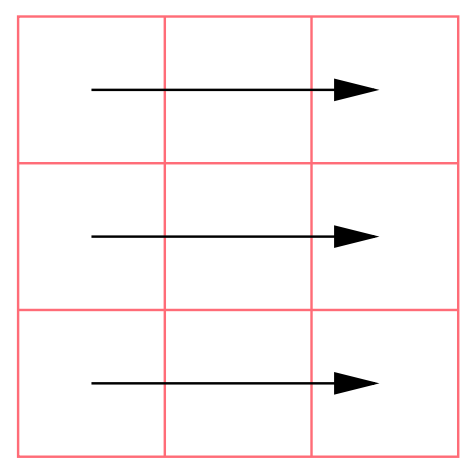
\includegraphics[width=4cm]{varredura.png} }}%
	\qquad
	\subfloat[\centering Direção de varredura da esquerda para direita com alternância (zig-zag)]{{ 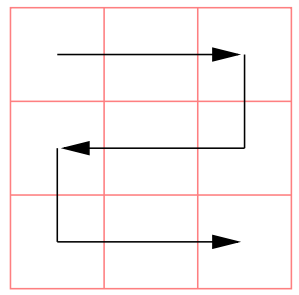
\includegraphics[width=4cm]{varredura_zigzag.png} }}%	
	\caption{Direção de varredura considerada para aplicação das técnicas de meios-tons (fonte: imagem extraida do documento pdf com as orientações deste trabalho).}%	
	\label{fig:direcao_varredura}%
\end{figure}

\noindent
Essas opções de varredura foram consideras porque a aparência visual das imagens resultantes se mostrou satisfatório, não havendo padrões estranhos que causassem desconforto ao olhar do observador.

Para o processo de aplicação das técnicas de meios-tons em imagens coloridas optou-se por trabalhar no mapa de cores HSV cujas letras são abreviações de \textit{Hue} (matiz), \textit{Saturation} (saturação) e \textit{Value} (valor). Assim, as imagens que, quando carregadas pelo opencv, eram disponibilizadas no mapa de cores BGR tiveram este mapa de cores convertido para o mapa HSV. Já no mapa de cores HSV, apenas o canal V (Value) da imagem (que é o que contém a intensidade luminosa) foi passado para as funções responsáveis pela aplicação das técnicas de meios-tons por difusão de erro. Obtido o canal V em meios-tons, este foi integrado ao esquema HSV original e a nova imagem foi reconvertida para o mapa de cores BGR.

Um dos destaques das implementações realizadas é a classe \textbf{Mask}. Essa classe ficou responsável pelo encapsulamento da lógica de recuperação dos pesos das mascaras das técnicas de meios-tons por difusão de erro bem como das posições nas quais estes pesos devem ser aplicados na imagem original. Dessa maneira, para o usuário, só ficou necessário passar a matriz da mascara da técnica de meio-tom em questão e a posição de referência do posicionamento na mascara do pixel \textbf{f(x,y)} da imagem original. Essa classe foi implementada como um objeto \textbf{iterador} do Python de modo que a obtenção dos pesos bem como da posição de aplicação destes na imagem original era facilmente alcançada dentro de uma estrutura de laço de repetição. Isso tornou bastante conveniente a integração da instancia da classe \textbf{Mask} dentro da função responsável por construir a imagem \textbf{g(x, y)} possuidora dos pixels em meios-tons. A implementação da classe \textbf{Mask} é apresentada a baixo.

\begin{lstlisting}
class Mask:
  def __init__(self, mask):
    self.name = mask.name
    self.mask = mask.mask
    self.ref = mask.ref


  def __iter__(self):
    self._r = 0
    self._c = -1 
    return self


  def __next__(self):
    mask = self.mask
    row, col = mask.shape
    _r = self._r; _c = self._c

    _c += 1
    if _c == col:
      _r += 1 
      _c = _c % col

    while True:
      if _r < row:
        val = mask[_r][_c]

        if val:
          self._r = _r
          self._c = _c
          inc = (_r - self.ref[0] , _c - self.ref[1], )
          return val, inc # retorna o peso a ser multiplicado pelo erro e o incremento
                          # a ser adicionando no pixel (x,y) da imagem f para difusao
                          # do erro

        _c += 1
        if _c == col:
          _r += 1 
          _c = _c % col

      else:
        break

  raise StopIteration
\end{lstlisting}

Para demais informações acerca das implementações ou algoritmos utilizados, consultar o código fonte. Lá existem comentários que abrangem esse tipo de informação.

%
%%
\section{Resultado}
Os resultados levantados são provenientes da aplicação do programa \textbf{main.py} sobre as imagens apresentadas na Figura \ref{fig:imagem:entrada}. 

\begin{figure}[!htp]%
	\centering
	\subfloat[\centering Vesão colorida da imagem Baboon (original)]{{ 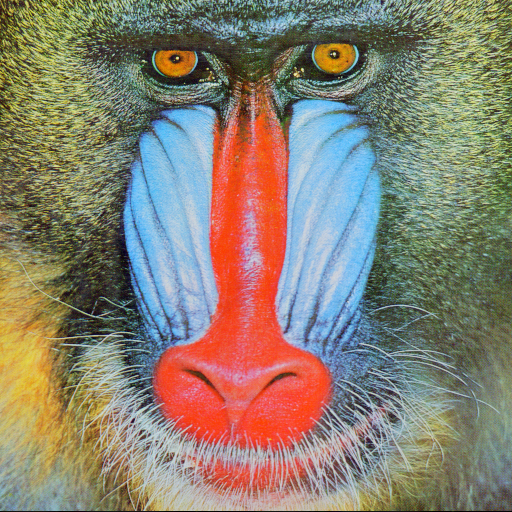
\includegraphics[width=5cm]{../out/cbaboon.png} }}%
	\qquad
	\subfloat[\centering Versão em escala de cinza da imagem Baboon (convertida)]{{ 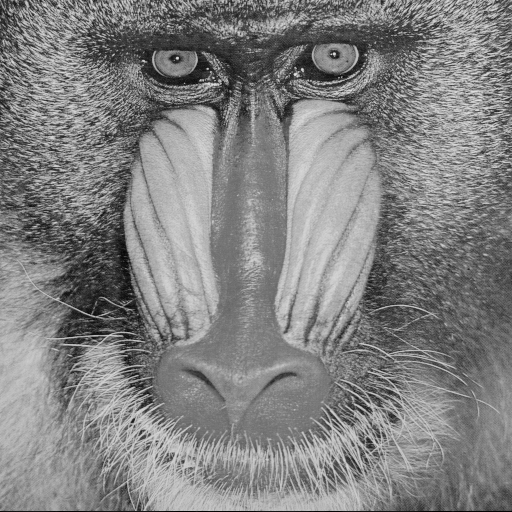
\includegraphics[width=5cm]{../out/baboon.png} }}%	
	\caption{Imagens utilizadas para aplicação das técnicas de meios-tons por difusão de erro.}%	
	\label{fig:imagem:entrada}%
\end{figure}

Para comparação com as imagens resultantes das técnicas de meios-tons por difusão de erro, gerou-se imagens denominadas controle a partir da aplicação da técnica de meio-tom que utiliza apenas o limiar de 128 para tomada de decisão se a um pixel será atribuído o valor zero (0) ou o valor (1). As imagens controle da imagem Baboon nas versões colorida e em escala de cinza são apresentadas na Figura \ref{fig:imagem:controle}.

\begin{figure}[!htp]%
	\centering
	
	\subfloat[\centering Imagem controle na versão colorida]{{ 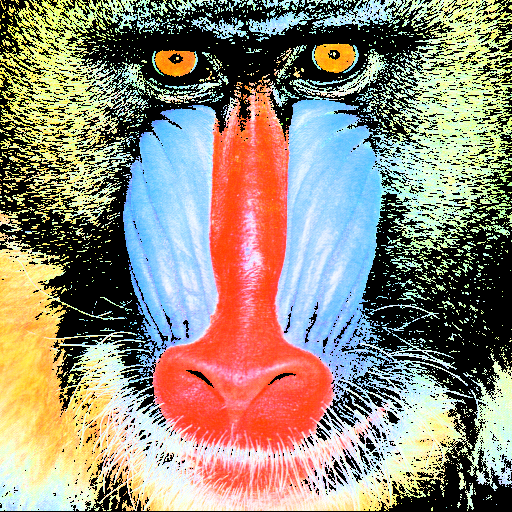
\includegraphics[width=5cm]{../out/cbaboon_control.png} }}%
	\qquad
	\subfloat[\centering Imagem controle na versão em preto e branco]{{ 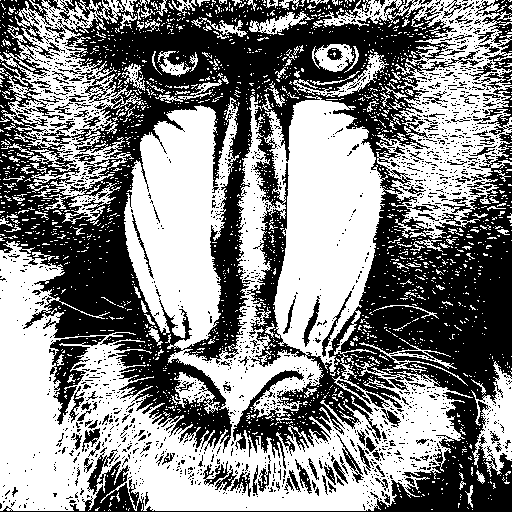
\includegraphics[width=5cm]{../out/baboon_control.png} }}%	
	
	\caption{Imagens controle para comparação com as imagens resultantes da aplicação da técnicas de meios-tons por difusão de erro.}%
	
	\label{fig:imagem:controle}%
\end{figure}

Na sequência, teremos a apresentação das imagens resultantes da aplicação das técnias de meios-tons por difusão de erro sobre a imagem Baboon na sua versão colorida e em escala de cinza.

%
\subsection{Técnicas de meios-tons sobre images em escala de cinza (varredura \textit{default})}
Aqui serão apresentados as imagens resultantes da aplicação das técnicas de meios-tons sobre a imagem de entrada em escala de cinza.

\begin{figure}[!htp]%
	\centering
	\subfloat[\centering Imagem em meio-tom pela técnica de Floyd e Steinberg]{{ 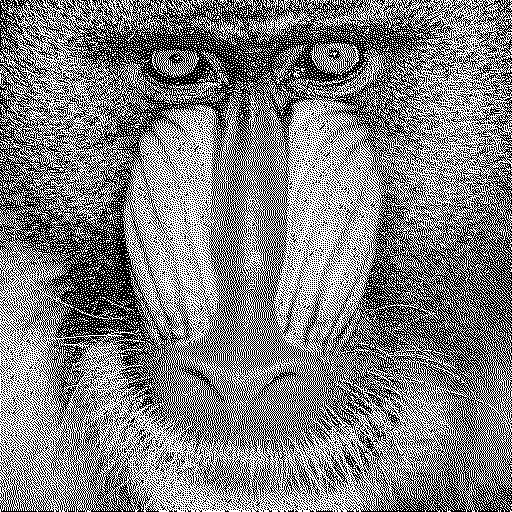
\includegraphics[width=3cm]{../out/baboon_floydsteinberg.png} }}%
	\qquad
    \subfloat[\centering Imagem em meio-tom pela técnica de Stevenson e Arce]{{ 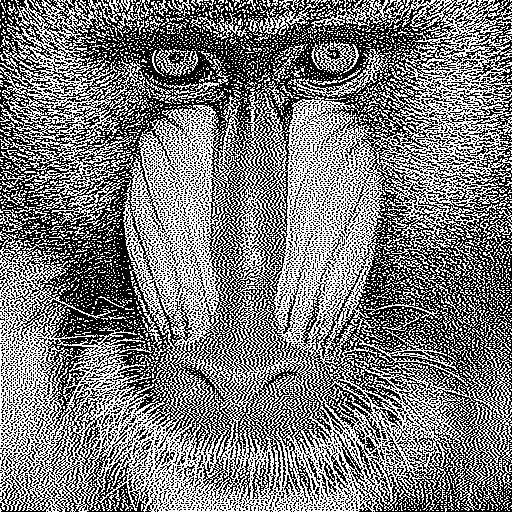
\includegraphics[width=3cm]{../out/baboon_stevensonarce.png} }}%
	\qquad
    \subfloat[\centering Imagem em meio-tom pela técnica de Burkers]{{ 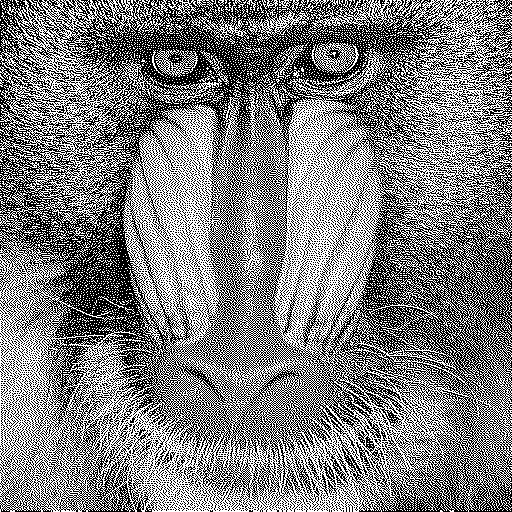
\includegraphics[width=3cm]{../out/baboon_burkers.png} }}%

	\subfloat[\centering Imagem em meio-tom pela técnica de Sierra]{{ 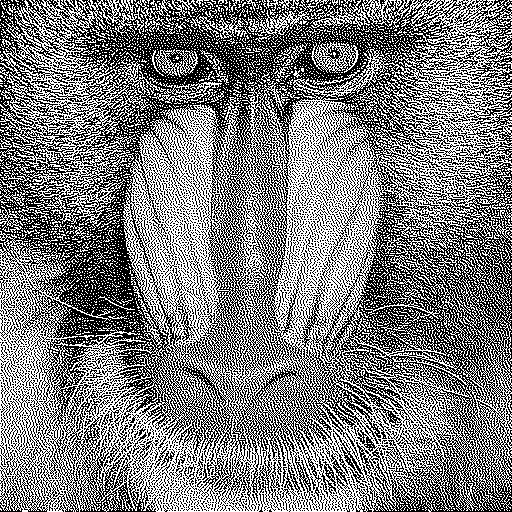
\includegraphics[width=3cm]{../out/baboon_sierra.png} }}%
    \qquad
   	\subfloat[\centering Imagem em meio-tom pela técnica de Stucki]{{ 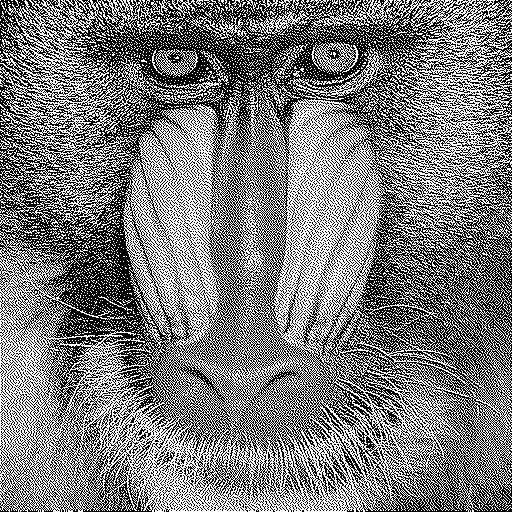
\includegraphics[width=3cm]{../out/baboon_stucki.png} }}%
   	\quad
 	\subfloat[\centering Imagem em meio-tom pela técnica de Javis, Judice e Ninke]{{ 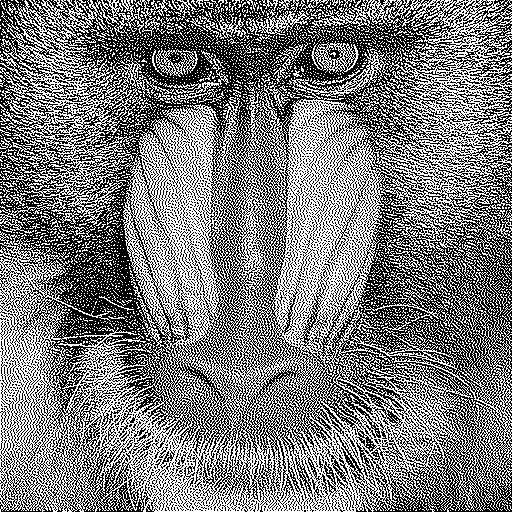
\includegraphics[width=3cm]{../out/baboon_jarvis.png} }}%
	
	\caption{Imagens resultantes em escala de cinza da aplicação das técnicas de meios-tons por difusão de erro em questão usando a varredura \textit{default}.}%
	\label{fig:imagem:plano:baboon:cinza:1}%
\end{figure}	

%
\subsection{Técnicas de meios-tons sobre images em escala de cinza (varredura zig-zag)}
Aqui serão apresentados as imagens resultantes da aplicação das técnicas de meios-tons sobre a imagem de entrada em escala de cinza.

\begin{figure}[!htp]%
	\centering
	\subfloat[\centering Imagem em meio-tom pela técnica de Floyd e Steinberg]{{ 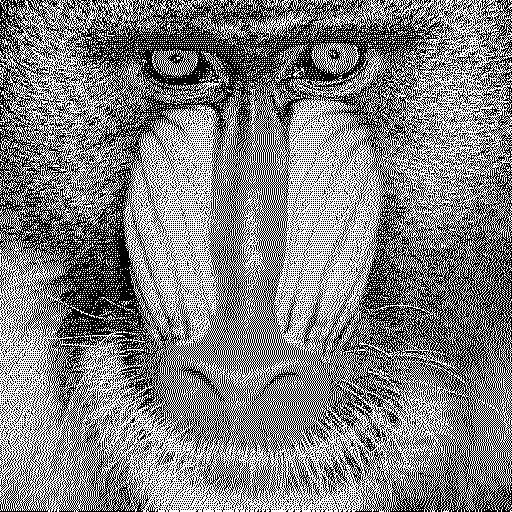
\includegraphics[width=3cm]{../out/zbaboon_floydsteinberg.png} }}%
	\qquad
	\subfloat[\centering Imagem em meio-tom pela técnica de Stevenson e Arce]{{ 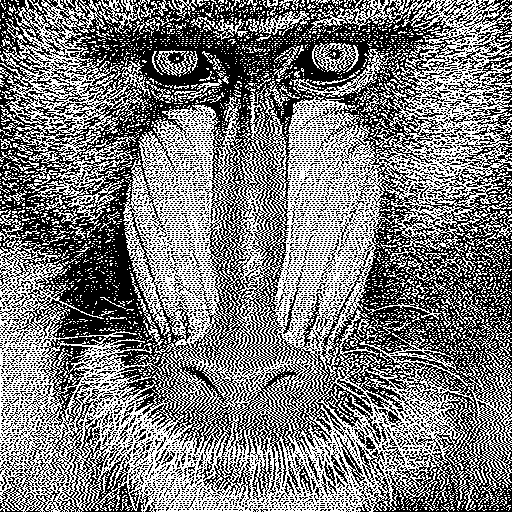
\includegraphics[width=3cm]{../out/zbaboon_stevensonarce.png} }}%
	\qquad
	\subfloat[\centering Imagem em meio-tom pela técnica de Burkers]{{ 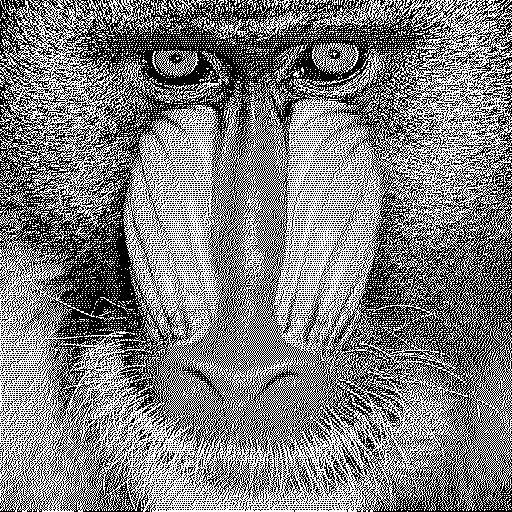
\includegraphics[width=3cm]{../out/zbaboon_burkers.png} }}%
	
	\subfloat[\centering Imagem em meio-tom pela técnica de Sierra]{{ 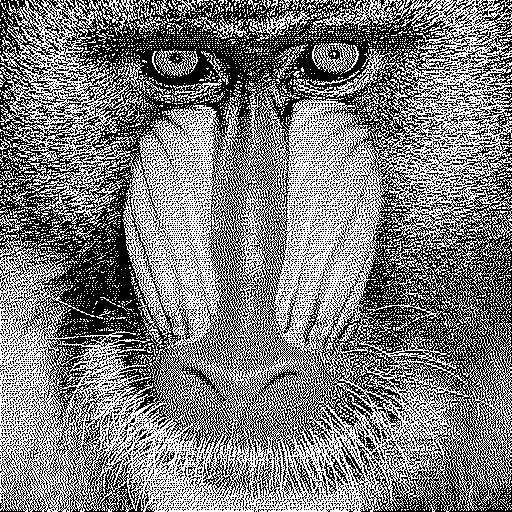
\includegraphics[width=3cm]{../out/zbaboon_sierra.png} }}%
	\qquad
	\subfloat[\centering Imagem em meio-tom pela técnica de Stucki]{{ 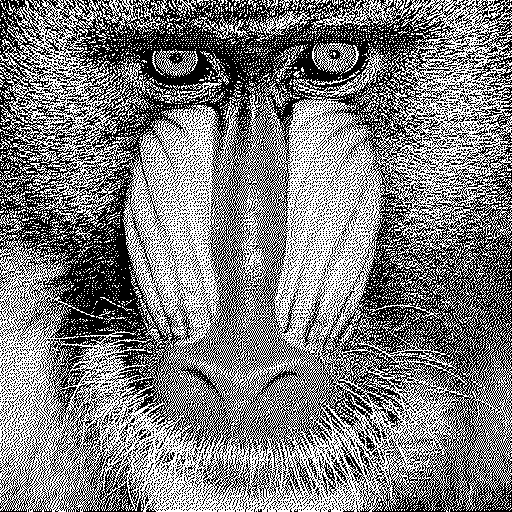
\includegraphics[width=3cm]{../out/zbaboon_stucki.png} }}%
	\quad
	\subfloat[\centering Imagem em meio-tom pela técnica de Javis, Judice e Ninke]{{ 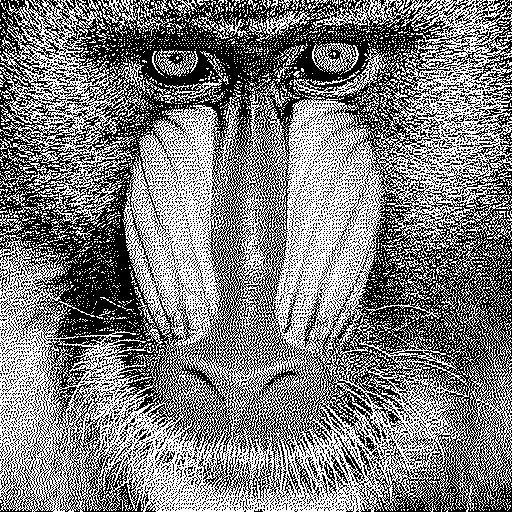
\includegraphics[width=3cm]{../out/zbaboon_jarvis.png} }}%
	
	\caption{Imagens resultantes em escala de cinza da aplicação das técnicas de meios-tons por difusão de erro em questão usando a varredura zig-zag.}%
	\label{fig:imagem:plano:baboon:cinza:2}%
\end{figure}	

%
\subsection{Técnicas de meios-tons sobre images coloridas (varredura \textit{default})}
Temos a seguir apresentadas as imagens resultantes da aplicação das técnicas de meios-tons sobre a imagem de entrada colorida.

\begin{figure}[!htp]%
	\centering
	\subfloat[\centering Imagem em meio-tom pela técnica de Floyd e Steinberg]{{ 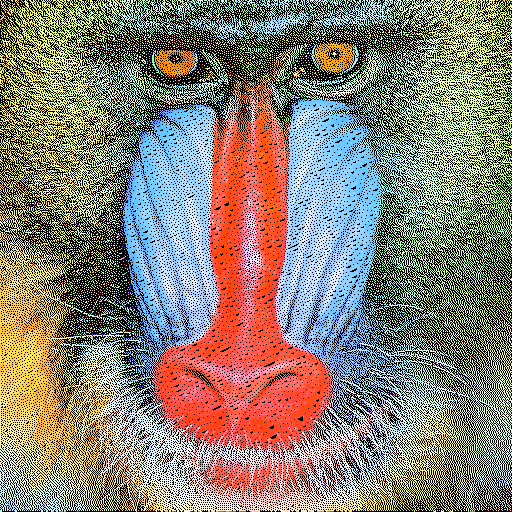
\includegraphics[width=3cm]{../out/cbaboon_floydsteinberg.png} }}%
	\qquad
	\subfloat[\centering Imagem em meio-tom pela técnica de Stevenson e Arce]{{ 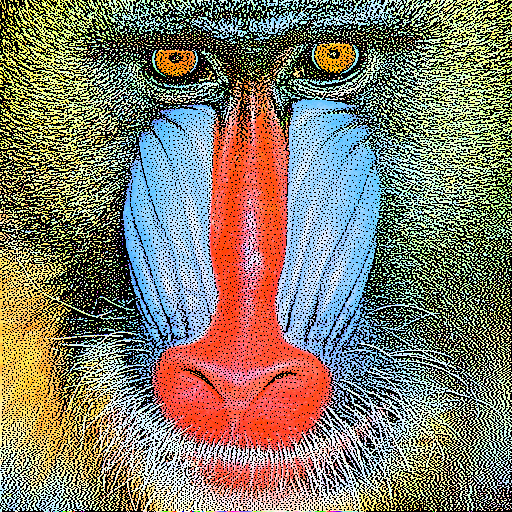
\includegraphics[width=3cm]{../out/cbaboon_stevensonarce.png} }}%
	\qquad
	\subfloat[\centering Imagem em meio-tom pela técnica de Burkers]{{ 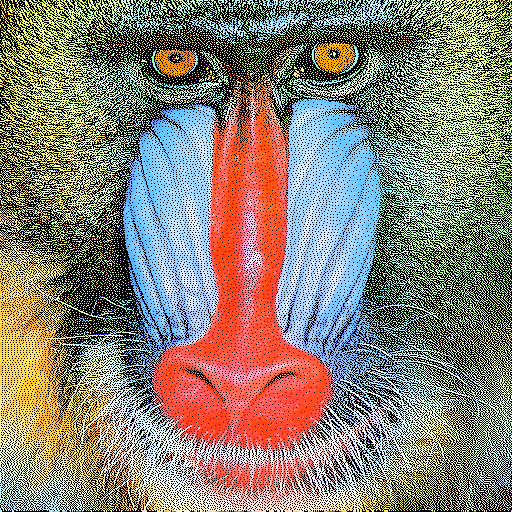
\includegraphics[width=3cm]{../out/cbaboon_burkers.png} }}%
	
	\subfloat[\centering Imagem em meio-tom pela técnica de Sierra]{{ 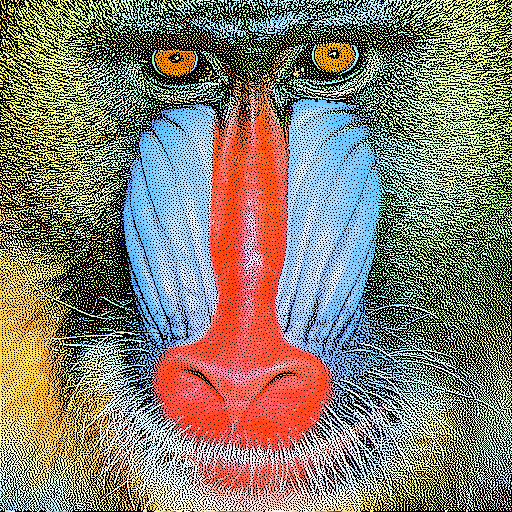
\includegraphics[width=3cm]{../out/cbaboon_sierra.png} }}%
	\qquad
	\subfloat[\centering Imagem em meio-tom pela técnica de Stucki]{{ 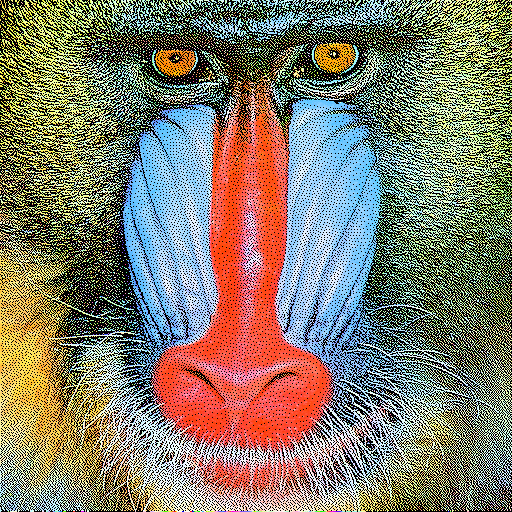
\includegraphics[width=3cm]{../out/cbaboon_stucki.png} }}%
	\quad
	\subfloat[\centering Imagem em meio-tom pela técnica de Javis, Judice e Ninke]{{ 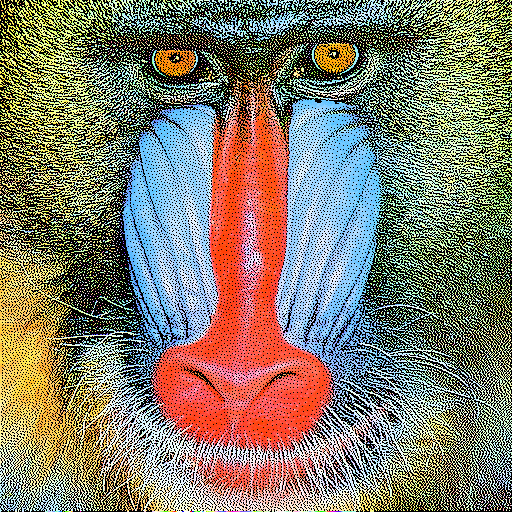
\includegraphics[width=3cm]{../out/cbaboon_jarvis.png} }}%
	
	\caption{Imagens resultantes coloridas da aplicação das técnicas de meios-tons por difusão de erro em questão usando a varredura \textit{default}.}%
	\label{fig:imagem:plano:baboon:colorido:1}%
\end{figure}


%
\subsection{Técnicas de meios-tons sobre images coloridas (varredura zig-zag)}
Temos a seguir apresentadas as imagens resultantes da aplicação das técnicas de meios-tons sobre a imagem de entrada colorida.

\begin{figure}[!htp]%
	\centering
	\subfloat[\centering Imagem em meio-tom pela técnica de Floyd e Steinberg]{{ 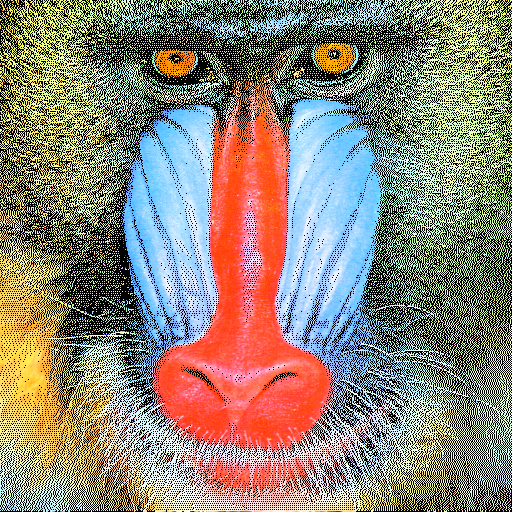
\includegraphics[width=3cm]{../out/czbaboon_floydsteinberg.png} }}%
	\qquad
	\subfloat[\centering Imagem em meio-tom pela técnica de Stevenson e Arce]{{ 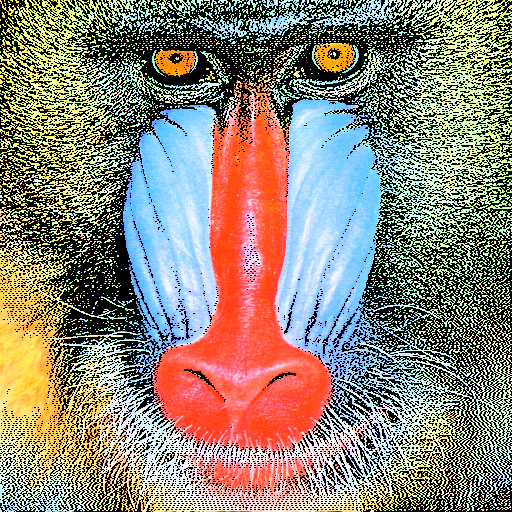
\includegraphics[width=3cm]{../out/czbaboon_stevensonarce.png} }}%
	\qquad
	\subfloat[\centering Imagem em meio-tom pela técnica de Burkers]{{ 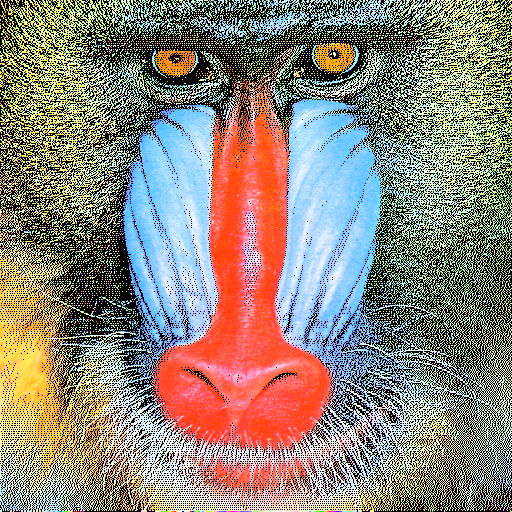
\includegraphics[width=3cm]{../out/czbaboon_burkers.png} }}%
	
	\subfloat[\centering Imagem em meio-tom pela técnica de Sierra]{{ 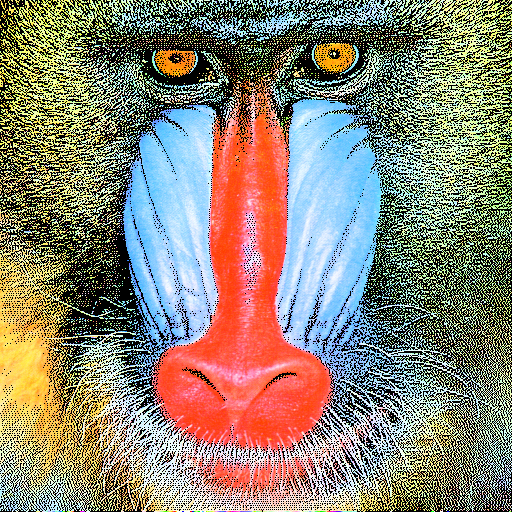
\includegraphics[width=3cm]{../out/czbaboon_sierra.png} }}%
	\qquad
	\subfloat[\centering Imagem em meio-tom pela técnica de Stucki]{{ 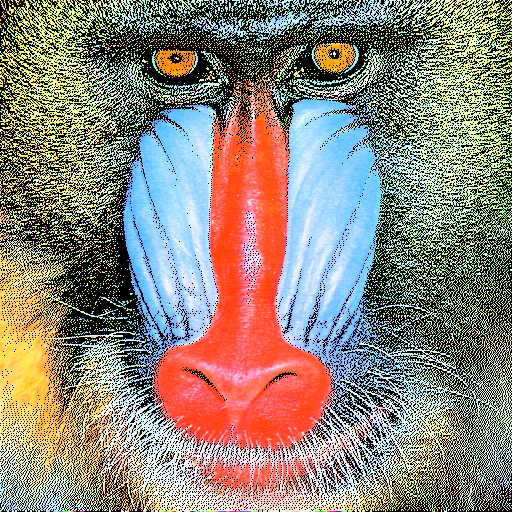
\includegraphics[width=3cm]{../out/czbaboon_stucki.png} }}%
	\quad
	\subfloat[\centering Imagem em meio-tom pela técnica de Javis, Judice e Ninke]{{ 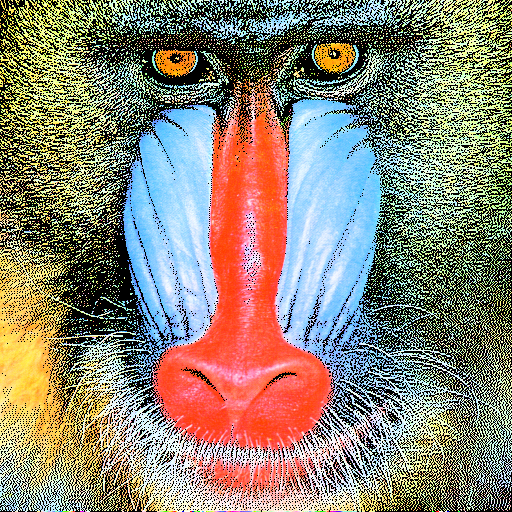
\includegraphics[width=3cm]{../out/czbaboon_jarvis.png} }}%
	
	\caption{Imagens resultantes coloridas da aplicação das técnicas de meios-tons por difusão de erro em questão usando a varredura zig-zag.}%
	\label{fig:imagem:planocolorido:2}%
\end{figure}

\section{Dicussão e Conclusão}
Do apresentado, podemos concluir que as técnicas de meios-tons foram aplicadas satisfatoriamente tanto sobre imagens coloridas quanto sobre imagens em escala de cinza. Para a imagem utilizada e dentro das dimensões consideradas, as ténicas de meios-tons tiveram resultados visuais semelhantes e bastante satisfatórios. Agora, dentro de uma análise mais minuciosa (ampliando-se as imagens) a técnica de meio-tom de Floyd e Steinberg apresentou uma imagem resultante com algumas falhas e vazios pretos na imagem resultante que não foram apresentados pelas imagens resultantes da aplicação das outras técnicas de meios-tons. Desse modo, quanto ao criterio visual, pode-se afirmar que a técnica de meio-tom de Floyd Steinberg apresentou os resultados menos interessantes com relação a harmonia visual da imagem resultante. Por outro lado, a aplicação da técnica de meio-tom de Floyd Steinberg é a menos custosa computacionalmente, dado que dispõe da menor mascara.

Sobre as duas varreduras utilizadas, verifica-se que o resultante de ambas foi visualmente similar para a imagem utilizada. A diferença mais notável, foi que as imagens resultantes da aplicação das técnicas de meios-tons pela varredura em zig-zag ficaram com maior contraste que as imagens resultantes da varredura \textit{default}. Talvez para aplicações mais sofisticadas em que a qualidade das imagens em meios-tons seja crítica, a utilização de padrões de varredura mais complexos seja justificado, o que não é o caso dentro do contexto deste trabalho.

%Do apresentado neste trabalho, podemos concluir que a esteganografia é uma técnica interessante e promissora de ocultação de mensagens em imagens sem que estas apresentem modificações visuais ao olho humano. De qualquer maneira, mesmo que visualmente as imagens não sejam alteradas, verificamos que ainda sim é possível identificar que a imagem está modifica e, assim, possivelmente com alguma mensagem escondida. Neste trabalho, essa verificação foi feita pela análise dos planos de bits das imagens modificadas. Nesse verificação, foi possível visualizar uma alteração do padrão de bits do plano de bits 0 (plano onde foi inserida a mensagem) em ambas as imagens Baboon e Watch utilizadas. A única exceção aconteceu com a imagem Baboon e a mensagem escondida \textbf{texto1.txt} que se deu, principalmente, porque a mensagem utilizada é muito pequena.


\end{document}
